\section{Observation Model}

Consider $p( z_i | obj_c)$. We will assume that $\theta_i$ is known, and thus we
just need to model $p( r_i | obj_c, \theta_i)$. We will do this by building a
lookup table of histograms from simulated data.

We generate a number of simulated environments with objects placed in random
positions and orientations. We then generate simulated LIDAR data from this
environment.

We take each $z_i$ generated. We project each ray into the object's frame. We
compute the relative angle between the ray and the object, $\phi = \theta_i -
\theta_{object}$. We also compute the closest distance between the ray and the
center of the object location, $d_{\text{ray}}$. Finally, we compute
$d_{\text{obs}}$, the position of the range $r_i$ along the ray, relative to the
closest point along the ray to the object center. This is depicted in
\figref{fig:obs_model} and given by:
%
\begin{align}
  \phi            &= \theta_i  - \theta_{\text{object}}        \text{,} \\
  d_{\text{ray}}  &= x \sin(\theta_i) - y \cos(\theta_i)       \text{,} \\
  d_{\text{obs}}  &= r_i - x \cos(\theta_i) - y \sin(\theta_i) \text{.}
\end{align}
%
\begin{figure}
  \centering
  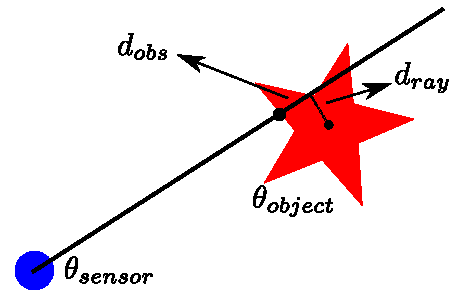
\includegraphics[width=2in]{figures/ray_model.pdf}
  \caption{Ray-based observation model for a given object. The sensor is
    depicted by the blue circle. The red star depicts the object we are
    interested in.}
  \label{fig:obs_model}
\end{figure}
%
Thus, $(\phi, d_{\text{ray}})$ parameterizes the ray for the $z_i$ that we are
considering, and $d_{\text{obs}}$ represents the observation, relative to the
object's location. (Note that these can be positive or negative). So, we have
%
\begin{align}
  p( r_i | obj_c, \theta_i) &=
    p_{obj_c}( d_{\text{obs}} | \phi, d_{\text{ray}} )
  \text{.}
\end{align}
%
(Note that for the change of variables, $\frac{d}{d d_{\text{obj}}} r_i = 1$)

We maintain a two-dimensional array of histograms, parameterized by $(\phi,
d_{\text{ray}})$. We discretize $\phi$ at \unit{0.10}{\rad} and
$d_{\text{ray}}$ at \unit{0.10}{\m}. When building the observation model, for
each $z_i$, we find the appropriate histogram and update it with
$d_{\text{obs}}$.

Thus, \eqnref{eq:obj_model} becomes:
%
\begin{align}
  \log p( obj_c | \mathbf{Z} ) &=
   \log{\eta} + \sum_{i=1}^{n} { \log p_{obj_c}( d_{\text{obs}} | \phi, d_{\text{ray}}) }
   + \log p(obj_c)
   \text{,}
   \label{eq:obj_model_pos}
\end{align}

We assume that at any given location $(x, y)$, there can only be one object
across all classes (including the no object class) and orientations:
%
\begin{align}
  \sum_{ \text{class $c$, orientation $\theta_{\text{object}}$} }
  p(obj_c | \mathbf{Z})
  &= 1
\end{align}
%
Thus, we can compute $\log \eta$ and then $p(obj_c | \mathbf{Z})$ for all
classes and orientations.

We can visualize the result of these histograms by querying the log probability
of a potential LIDAR observation given a object of a certain class with a
certain state. This is depicted in \figref{fig:star_model} and
\figref{fig:box_model}.
%
\begin{figure*}
  \centering
  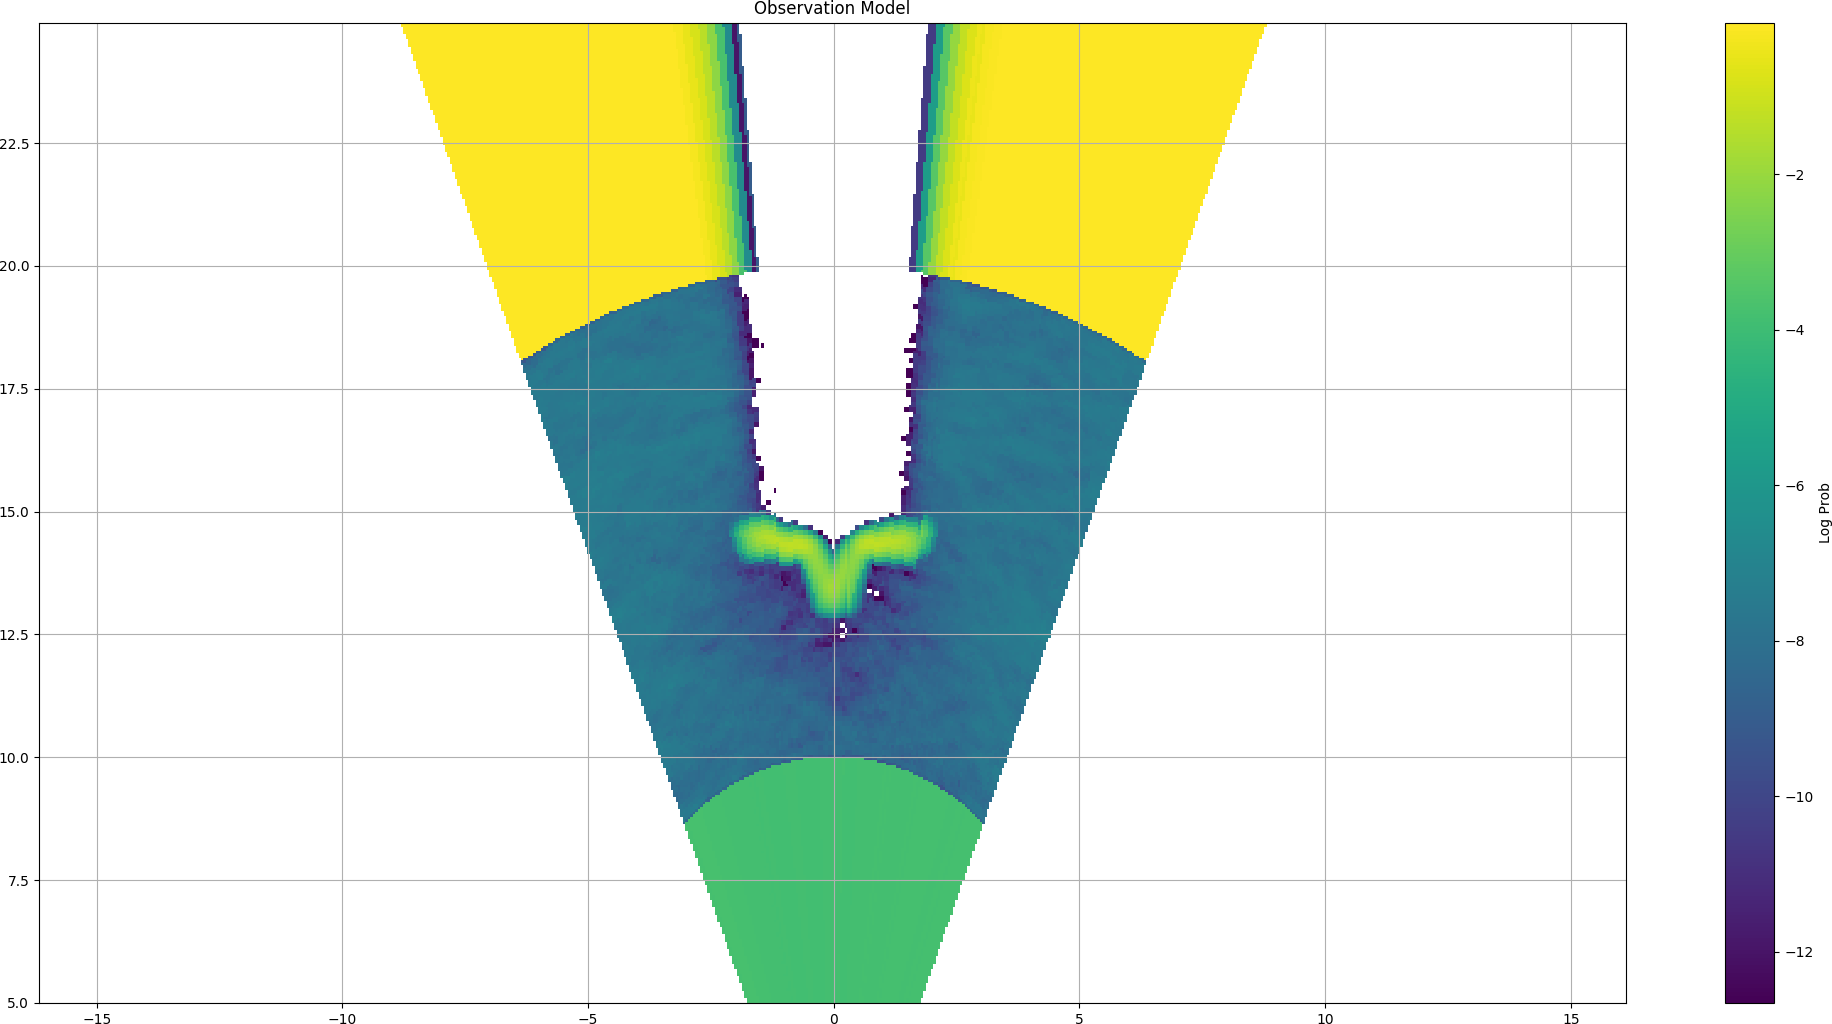
\includegraphics[width=\textwidth]{figures/star_model.png}
  \caption{Log probability of potential LIDAR observations from (0, 0) with a
    star placed at (0, 15). This is implemented as a lookup table of histograms.}
  \label{fig:star_model}
\end{figure*}
%
\begin{figure*}
  \centering
  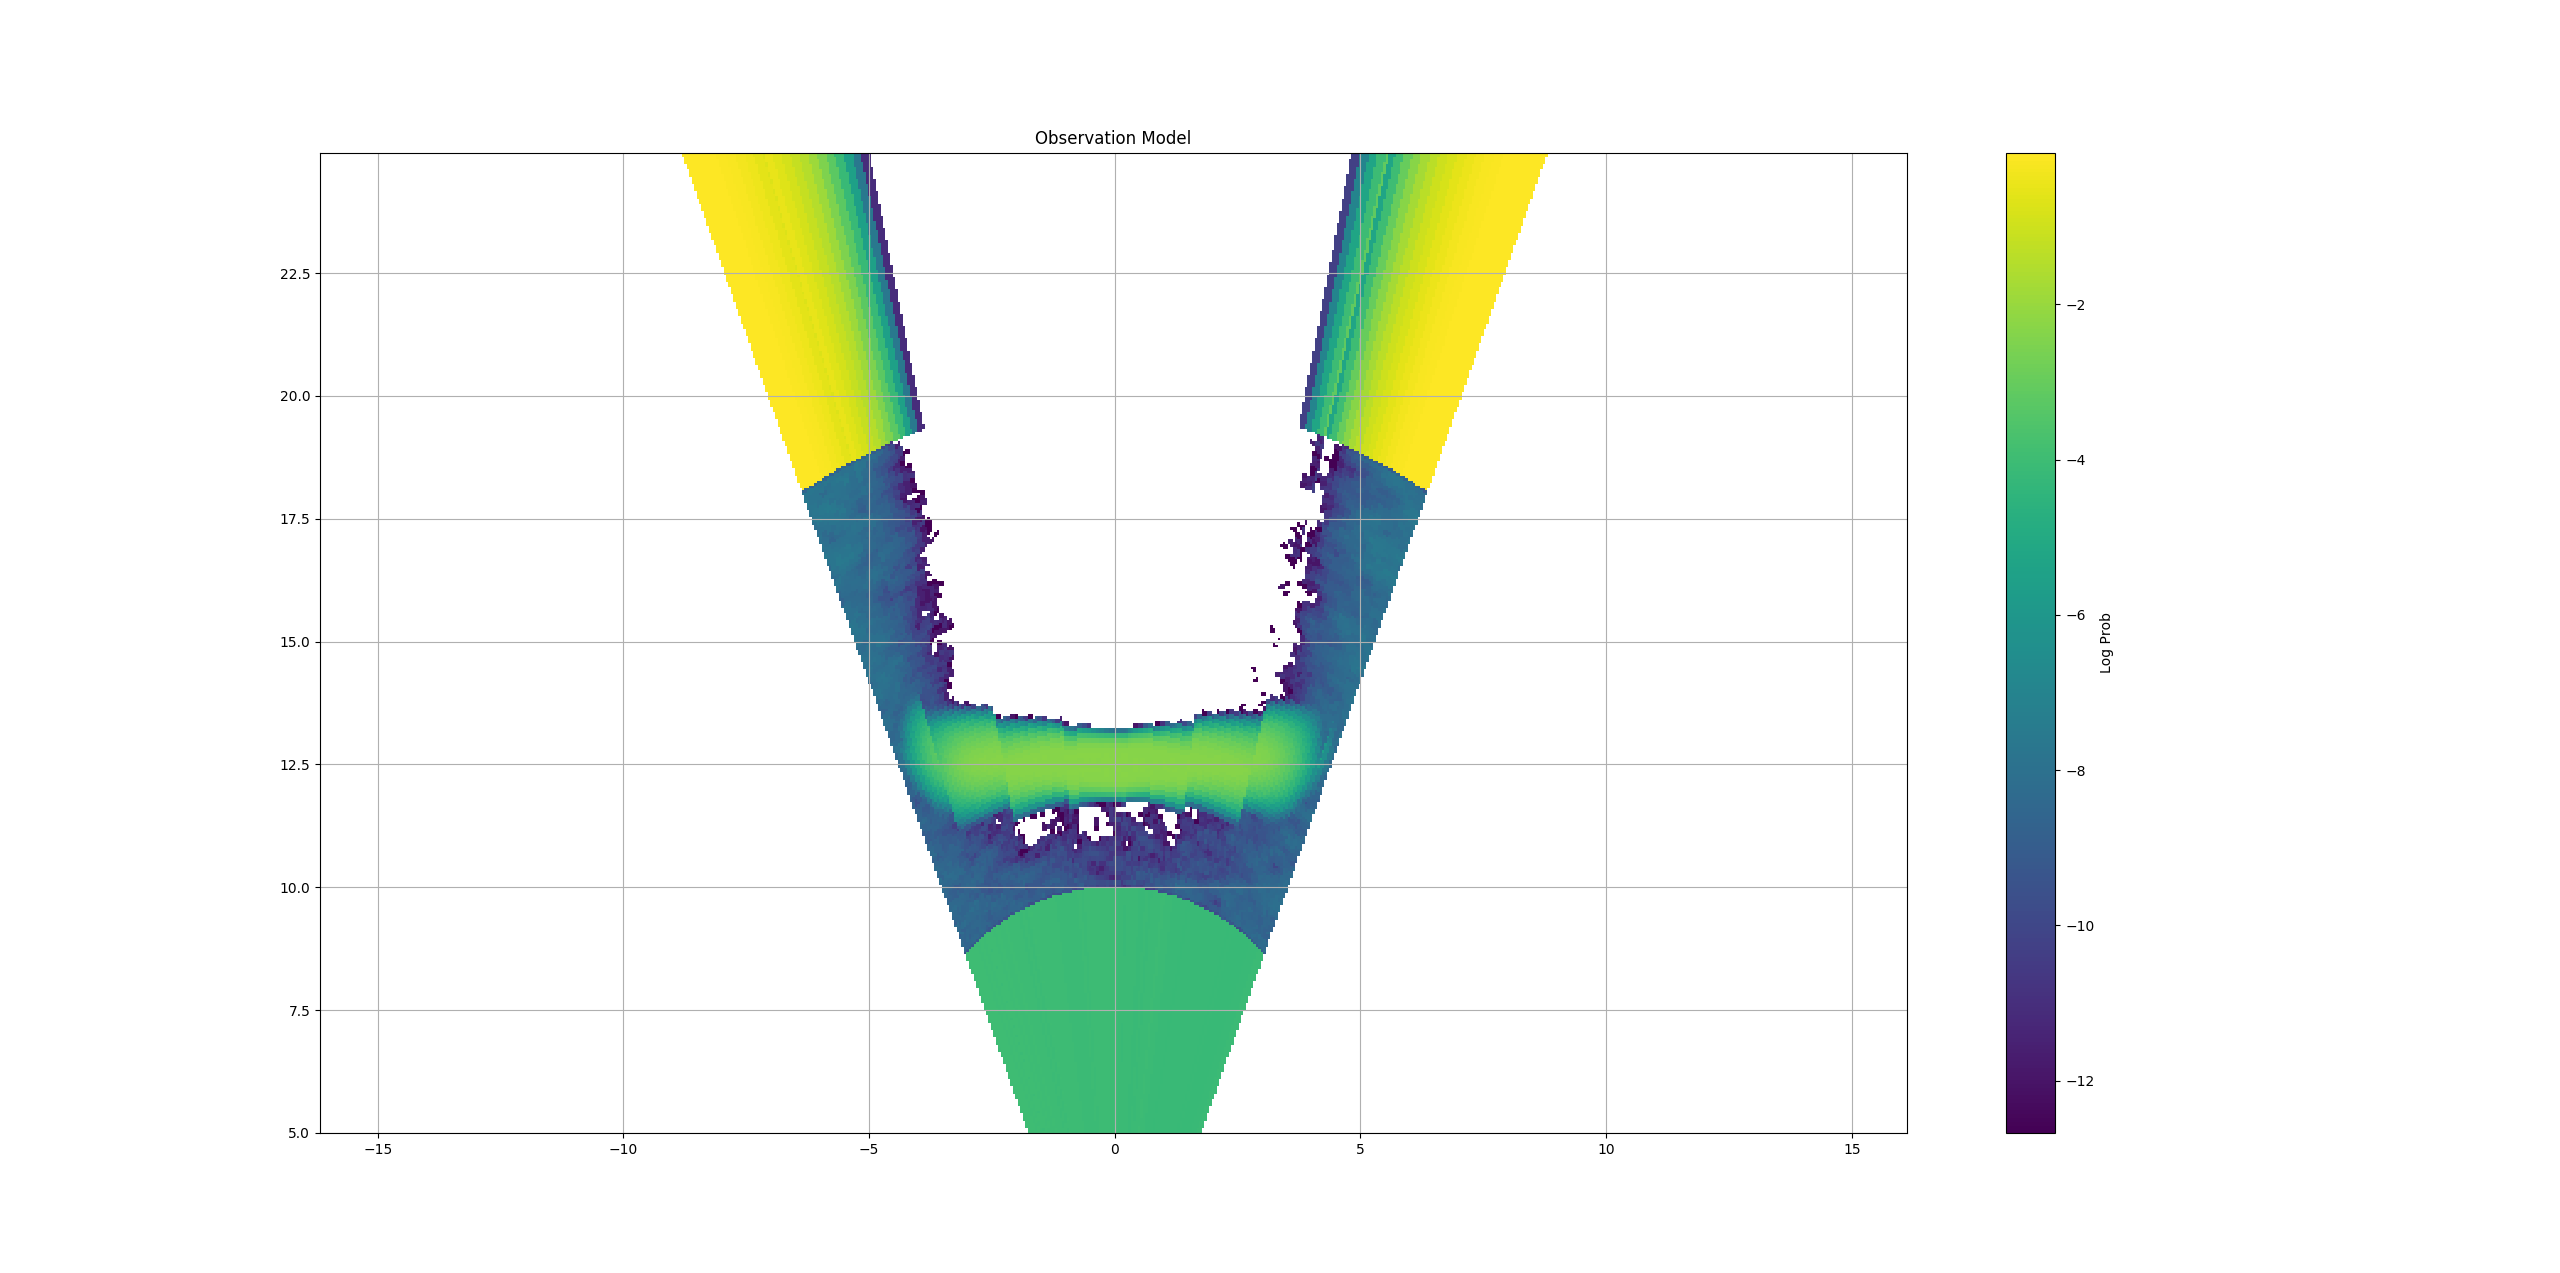
\includegraphics[width=\textwidth]{figures/box_model.png}
  \caption{Log probability of potential LIDAR observations from (0, 0) with a
    box placed at (0, 15). This is implemented as a lookup table of histograms.}
  \label{fig:box_model}
\end{figure*}
